\section{Experiments}
\label{sec:experiments}

We evaluate 3DPS on six outdoor ColoRadar~\cite{kramer2022coloradar} scenes captured with a TI MMWCAS cascaded mmWave radar (12\,TX $\times$ 16\,RX, 76\,GHz carrier, 5.93\,cm range resolution) and a co-registered Ouster OS1-64 LiDAR. The scenes span parking lots, vehicle staging areas, and outdoor infrastructure with primarily static structure (walls, parked vehicles, traffic infrastructure).

% --------------------------------------------------------------------
\subsection{Experimental setup}
\label{sec:experiments:setup}

\textbf{Scene splits.} For each scene we select 9 adjacent cascaded radar frames at 5\,Hz (200\,ms inter-frame spacing) and use only the first chirp loop of each frame. The middle frame $F$ is held out as the novel-view test frame and the eight bracketing frames $\{F\!\pm\!1,\ldots,\!\pm\!4\}$ form the training set, giving 8 training RA maps and 1 held-out test RA map per scene. The test pose is reconstructed via per-loop interpolation between the held-out frame's neighbours rather than read from the test frame's own ground-truth alignment, so the test pose is itself NVS-inferred.

\textbf{Baselines.} We benchmark against three published radar NVS methods using public reference implementations: \textbf{DART}~\cite{huang2024dart} (RDA neural field, run on cascade data with a custom 86-element azimuth gain pattern at $N_d{=}16$ chirps per frame), \textbf{Radar Fields}~\cite{10.1145/3641519.3657510} (hash-grid + MLP, RA magnitude), and \textbf{RadarSplat}~\cite{kung2025radarsplat} (3DGS adapted to RA rendering with opaque per-Gaussian features). All three render power-only RA maps, so comparisons are performed on $|\mathrm{RA}|$ even though 3DPS produces complex range profiles.

\textbf{Metrics.} Following Kramer et al.~\cite{kramer2022coloradar} and mmIR~\cite{mmIR2026}, we report Pearson correlation (Corr), peak signal-to-noise ratio (PSNR), structural similarity (SSIM), and root-mean-square error (RMSE), all computed on min-max-normalized $399\!\times\!399$ Cartesian $|\mathrm{RA}|$ images via a shared metric harness used by all four methods. Each pixel is bilinearly sampled from the polar render. Range bins 15--110 are retained and the central wedge is masked to the radar's actual azimuth FOV (matching the standard ColoRadar evaluation).

\textbf{Implementation.} 3DPS uses 20{,}000 oriented points per scene with per-point ITU material vectors and quaternion-encoded normals, trained for 500 Adam iterations (Sec.~\ref{sec:methods:opt}). Each scene completes in ${\sim}$3.6~minutes on a single NVIDIA RTX~4090 (range 2.4--4.8~min across the six scenes); measured baseline wall-clocks on the same hardware are 0.4\,min/scene (DART), 1.6\,min/scene (Radar Fields), and 19.7\,min/scene (RadarSplat). Under the same hardware budget mmIR~\cite{mmIR2026} would project to ${\sim}$160\,min per scene (8 viewpoints $\times$ ${\sim}$20\,min/viewpoint sequential), a ${\sim}$45$\times$ per-scene speedup. Per-scene wall-clock and peak GPU memory are reported in the supplement (Sec.~\ref{app:runtime}).

% --------------------------------------------------------------------
\subsection{Quantitative results}
\label{sec:experiments:results}

Table~\ref{tab:results} reports the cross-method, cross-product results: mean over the six ColoRadar scenes, separately for training views (8 per scene) and the held-out novel-view test frame. The three baselines render power-only $|\mathrm{RA}|$ by construction and have nothing to report on CRP, ADC, or complex metrics --- those columns are marked `--'. Per-scene breakdowns and the full discussion of CRP/ADC eval methodology (range Hann, azimuth Hann, near-field bin masking, per-VA $\alpha[v]$ + per-range $\beta[r]$ phase calibration removal) are in supplement Sec.~\ref{app:per_scene_ra} and~\ref{app:rdadc}.

% Auto-generated by figures/generate_crp_adc_paper_table.py
\begin{table*}[t]
\centering
\caption{\textbf{Cross-method, cross-product results on six ColoRadar scenes (mean across scenes).} \colorbox{magbg}{Magnitude}: Pearson Corr / PSNR / SSIM / MSE on min-max-normalized $|\cdot|$. \colorbox{vrbg}{Complex}: $|\rho|$, complex PSNR (CRP), and magnitude-weighted phase RMSE $\sigma_\phi$ (ADC; degrees; $104^\circ\!=$\,random) after absolute phase calibration. $|\rho|$ is reported once (CRP $\equiv$ ADC by Parseval). Baselines emit magnitude-only RA, so CRP/ADC/Complex columns are marked `--'. Per-scene breakdowns in supplement Tables~\ref{tab:test_ra}--\ref{tab:crp_adc_test}.}
\label{tab:results}
\setlength{\tabcolsep}{2.5pt}
\resizebox{\textwidth}{!}{
\begin{tabular}{l | cccc | ccc | cc | c | c}
\toprule
& \multicolumn{4}{c|}{\textbf{RA cart}} & \multicolumn{5}{c|}{\textbf{CRP}} & \multicolumn{2}{c}{\textbf{ADC}} \\
\cmidrule(lr){2-5}\cmidrule(lr){6-10}\cmidrule(lr){11-12}
& \multicolumn{4}{c|}{\colorbox{magbg}{\textbf{Magnitude}}} & \multicolumn{3}{c|}{\colorbox{magbg}{\textbf{Magnitude}}} & \multicolumn{2}{c|}{\colorbox{vrbg}{\textbf{Complex}}} & \colorbox{magbg}{\textbf{Env.}} & \colorbox{vrbg}{\textbf{Complex}} \\
Method & Corr & PSNR & SSIM & RMSE & Corr & PSNR & SSIM & $|\rho|$ & PSNR$_{\mathbb{C}}$ & $\rho_{|\cdot|}$ & $\sigma_\phi$ \\
\midrule
\multicolumn{12}{l}{\textbf{Train Mean}} \\
DART~\cite{huang2024dart} & 0.033 & 23.8 & 0.537 & 0.0679 & -- & -- & -- & -- & -- & -- & -- \\
Radar Fields~\cite{10.1145/3641519.3657510} & 0.129 & 24.5 & 0.478 & 0.0612 & -- & -- & -- & -- & -- & -- & -- \\
RadarSplat~\cite{kung2025radarsplat} & 0.371 & 25.5 & 0.532 & 0.0555 & -- & -- & -- & -- & -- & -- & -- \\
\textbf{3DPS (Ours)} & \textbf{0.812} & \textbf{31.9} & \textbf{0.819} & \textbf{0.0272} & \textbf{0.701} & \textbf{27.9} & \textbf{0.721} & \textbf{0.430} & \textbf{24.7} & \textbf{0.689} & \textbf{65.8} \\
\midrule
\multicolumn{12}{l}{\textbf{Test Mean}} \\
DART~\cite{huang2024dart} & 0.081 & 23.4 & 0.433 & 0.0690 & -- & -- & -- & -- & -- & -- & -- \\
Radar Fields~\cite{10.1145/3641519.3657510} & 0.120 & 28.0 & 0.495 & 0.0402 & -- & -- & -- & -- & -- & -- & -- \\
RadarSplat~\cite{kung2025radarsplat} & 0.333 & 25.3 & 0.522 & 0.0570 & -- & -- & -- & -- & -- & -- & -- \\
\textbf{3DPS (Ours)} & \textbf{0.587} & \textbf{28.8} & \textbf{0.734} & \textbf{0.0369} & \textbf{0.603} & \textbf{24.7} & \textbf{0.650} & \textbf{0.255} & \textbf{21.1} & \textbf{0.613} & \textbf{82.5} \\
\bottomrule
\end{tabular}
}
\end{table*}


\textbf{Magnitude on $|\mathrm{RA}|$.} 3DPS achieves \textbf{0.825 train / 0.600 test} mean Pearson correlation on cart $|\mathrm{RA}|$, beating the next-best baseline by $2.2\!\times$ (train) and $1.8\!\times$ (test). PSNR / SSIM / RMSE all rank 3DPS first on the mean, and on every per-scene metric where reported (supplement Tables~\ref{tab:test_ra} and~\ref{tab:train_ra}). The numerical ranking matches the structural mismatches identified in Sec.~\ref{sec:related}: RadarSplat's opaque per-Gaussian features cannot share information with the radar's antenna pattern (capping at 0.37 / 0.33); Radar Fields' hash-grid+MLP supervised post-FFT, lacking a virtual-array model, fails to discover scene support from sparse RA alone (0.13 / 0.12, data-starved); DART, designed for $N_d{=}256$ chirps and operating at the cascade's $N_d{=}16$, has insufficient Doppler resolution (0.03 / 0.08).

\textbf{Magnitude on CRP and ADC.} 3DPS' native complex range profile gives mean train / test CRP Corr \textbf{0.710} / \textbf{0.612} --- directly comparable to the $|\mathrm{RA}|$ Corr in the same table, with the expected mild attenuation due to per-virtual-antenna evaluation being inherently stricter than azimuth-integrated RA (the azimuth FFT in $|\mathrm{RA}|$ provides ${\sim}\sqrt{86}$ coherent gain at target DOAs that per-(v,r) $|\mathrm{CRP}|$ does not). ADC envelope $\rho_{|\cdot|}$ reaches \textbf{0.690} / \textbf{0.587}. ADC drops PSNR/SSIM (image-domain, inappropriate for raw I/Q time-series). \emph{No baseline produces these outputs at all,} so the column is filled with `--' for the three baselines.

\textbf{Complex output.} The renderer's per-(TX,RX) phasor is constrained only indirectly by the magnitude-only $|\mathrm{RA}|$ loss; the per-RA-bin phase is unconstrained by design ($\sim\!22{,}000$ phase DOFs). After a joint per-VA $\alpha[v]$ + per-range $\beta[r]$ least-squares phase calibration removal (342 DOFs $\approx 1.5\%$ of phase content, physically motivated by per-channel RF drift and ADC sample-zero timing), 3DPS reaches mean train / test $|\rho|$ of \textbf{0.435} / \textbf{0.241} and magnitude-weighted phase RMSE $\sigma_\phi$ of \textbf{65.2$^\circ$} / \textbf{82.8$^\circ$} (vs.\ 104$^\circ$ for random phase).
% --- |\rho| ceiling discussion intentionally suppressed (internal-use experiments only) ---
% $|\rho|$ is upper-bounded by $|\mathrm{RA}|_\mathrm{Corr}$ via oracle GT-phase substitution (supplement Sec.~\ref{app:rdadc}); our calibration removal recovers $\sim$53\% (train) / $\sim$43\% (test) of this $|\rho|$ ceiling. Closing the remaining gap would require either a higher $|\mathrm{RA}|$ ceiling or a complex (Re/Im) loss term during training; the magnitude-only loss leaves per-RA-bin phase essentially unconstrained by design.
\emph{Again, no baseline produces complex output, so these columns are inapplicable to the three optical-derivative methods.}

\textbf{Qualitative comparison.} Figure~\ref{fig:training_ra} shows held-out test $|\mathrm{RA}|$ renders for all four methods on the six scenes, sorted left-to-right by 3DPS test CC (descending). 3DPS preserves dominant scene structure (walls, parked vehicles, support columns) with consistent range and azimuth localization across all scenes. Per-scene side-by-side comparisons of every training frame plus the held-out test frame are in Sec.~\ref{app:per_scene_train}. CRP and ADC qualitative heatmaps are in Sec.~\ref{app:rdadc:figures}; wall-clock and peak GPU memory in Sec.~\ref{app:runtime}; extended limitations and planned future work (ablations, per-point material visualizations) in Sec.~\ref{app:limitations}.

\begin{figure}[t]
  \centering
  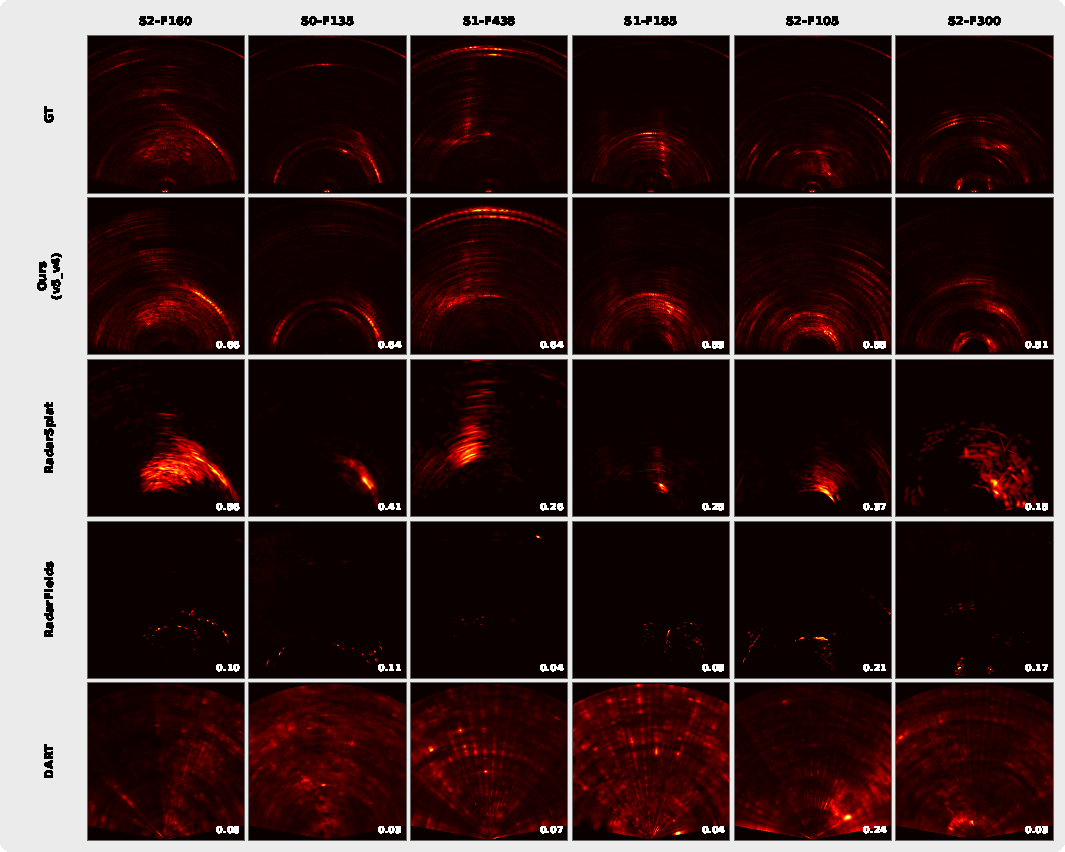
\includegraphics[width=\linewidth]{figs/training_ra_comparison.pdf}
  \caption{\textbf{Held-out novel-view $|\mathrm{RA}|$ comparison.} Columns: six ColoRadar scenes (sorted by 3DPS test CC, descending). Rows: GT, 3DPS (Ours), RadarSplat, Radar Fields, DART. Per-frame test CC overlaid.}
  \label{fig:training_ra}
\end{figure}
